%! Author = wolfram_e_laube
%! Date = 06.05.24

\item[(a)]
Below is the Python code for this exercise:

\begin{verbatim}
import numpy as np
import matplotlib.pyplot as plt

# Given parameters
fs = 8e3  # Sampling frequency in Hz
frequencies = np.array([2e3, 5e3])  # Example frequencies in Hz (assumption)

# Part (a) and (b)
def plot_spectrum(frequencies, fs):
    # Shift frequencies by -fs, 0, and +fs
    shifts = [-fs, 0, fs]
    shifted_freqs = [frequencies + s for s in shifts]

    plt.figure()
    for s_freqs, s in zip(shifted_freqs, shifts):
        for freq in s_freqs:
            plt.axvline(x=freq / 1e3, linestyle='-', color='b')
            plt.axvline(x=-freq / 1e3, linestyle='-', color='b')

    plt.xlabel('Frequency (kHz)')
    plt.ylabel('Amplitude')
    plt.title('Spectrum with Sampling')
    plt.grid(True)
    plt.xlim(-12, 12)  # Adjust according to the actual range
    plt.show()

# Plot the spectrum
plot_spectrum(frequencies, fs)
\end{verbatim}

\begin{figure}[h]
    \centering
    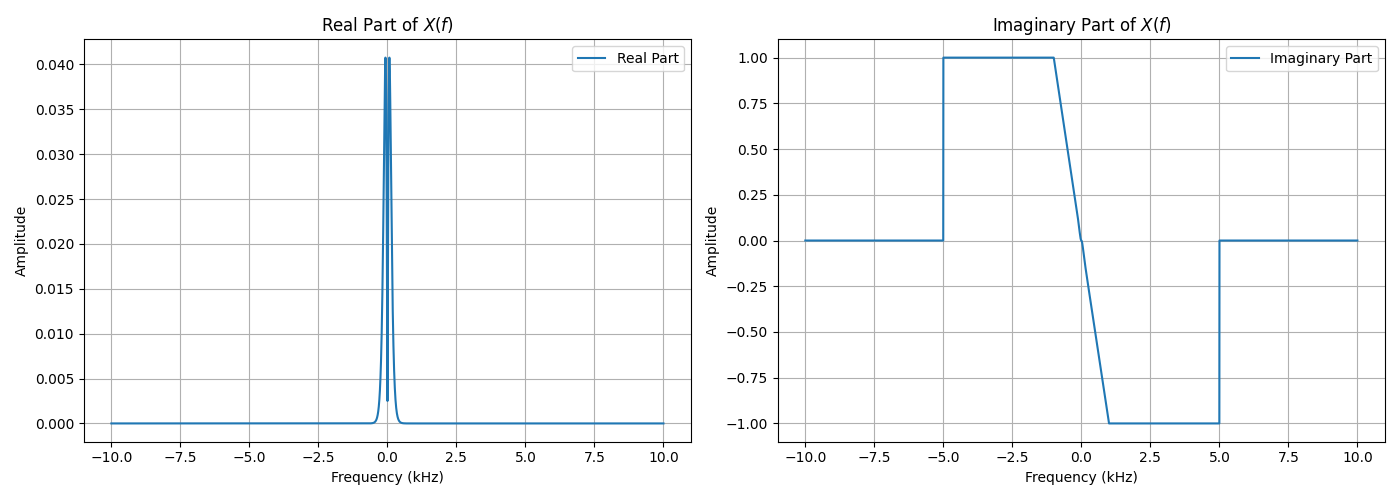
\includegraphics[width=0.49\textwidth]{fig/ex2_a_plot}
    \caption{Spectrum of \(x(t)\)}
    \label{fig:ex2_a_plot}
\end{figure}
